Monissa käytännön tilanteissa jokin suure voidaan päätellä tai laskea kahdella eri tavalla. Nämä tavat voidaan merkitä lukuina tai kirjoittaa lausekkeiksi. Merkitsemällä näin saadut lukuarvot ja lausekkeet yhtäsuuriksi saadaan \termi{yhtälö}{yhtälö}. Yhtälö on siis kahden lausekkeen merkitty yhtäsuuruus. Monia käytännön tilanteita voidaan mallintaa käyttämällä yhtälöitä.

\begin{esimerkki}
	Merkitään lausekkeet $5x+\sqrt{x}$ ja $7x+7$ yhtäsuuriksi, jolloin saadaan yhtälö $5x+\sqrt{x} = 7x+7$.
\end{esimerkki}

\laatikko{
	Jos yhtälön kummankin puolen lausekkeen arvo on sama, sanotaan että \termi{yhtälön päteminen}{yhtälö pätee}.
}

\begin{esimerkki}
	\begin{alakohdat}
		\alakohta{Yhtälö $3x + 2 = 0$ pätee, kun $x = - \frac{2}{3}$.}
		\alakohta{Yhtälö $5 = 3$ ei päde.}
	\end{alakohdat}
\end{esimerkki}


\laatikko[Yhtälöihin liittyviä termejä]{
	\begin{description}
		\item[Tuntematon] Luku, jonka arvoa ei tiedetä. Tuntemattomia merkitään vaihtelevilla symboleilla. Jos tuntemattomia on vain yksi, sitä merkitään 	yleensä kirjaimella $x$.
		\item[Yhtälön ratkaisu] Tuntemattoman $x$ arvo, jolla yhtälö pätee.
		\item[Yhtälön ratkaiseminen] Kaikkien yhtälön ratkaisujen selvittäminen.
	\end{description}
	
}

Huomioi, että yhtälössä voi olla useitakin eri tuntemattomia. 

%Lisännyt Jaakko Viertiö 2013-11-10
\begin{esimerkki}
 Tarkastellaan yhtälöä $x^3-2x^2-x+2=0$. Yhtälön \textit{eräs} ratkaisu on $x=1$, sillä $1^3-2\cdot{1^2}-1+2=0$. 
 Myös $x=2$ on kyseisen yhtälön ratkaisu, sillä $2^3-2\cdot{2^2}-2+2=0$. 
 Tuntemattomalle $x$ voidaan siis joissain tapauksissa löytää useita arvoja, jotka toteuttavat yhtälön. 
\end{esimerkki}

% FIXME: jokin helposti ymmärrettävä esimerkki tuntemattomista

Tyypillinen tapa ratkaista yhtälöitä on kirjoittaa ne ilmaistuna toisella tavalla.
Käytännössä tämä tarkoittaa niiden muokkaamista siten, ettei alkuperäisen yhtälön paikkansapitävyys muutu.
%Lisännyt Jaakko Viertiö 2013-11-10. Rautalangasta aina paras!
Yleensä tavoitteena on saada yhtälö muotoon, jossa yhtäpitävyyden toisella puolella on vain haluttu muuttuja ilman kertoimia, ja toisella puolella kaikki muu.

\laatikko[Yhtälöiden muokkaaminen]{
	\begin{description}
		\item[Puolittain lisääminen tai vähentäminen] Yhtälön molemmille puolille voidaan lisätä tai molemmilta puolilta voidaan vähentää luku. Esimerkiksi yhtälö $3x+5 = 3$ saadaan näin muotoon $3x = -2$.
		\item[Puolittain kertominen tai jakaminen] Yhtälön molemmat puolet voidaan kertoa tai jakaa nollasta poikkeavalla luvulla. Esimerkiksi kertomalla yhtälön $2x = 4$ molemmat puolet luvulla $\frac{1}{2}$ saadaan yhtälö $x = 2$.
	\end{description}
%Huomautuksen ja jakolaskumaininnan lisännyt Jaakko Viertiö 2013-11-10
	Huomaa, että itseasiassa vähennyslasku on negatiivisen luvun summaamista [$a-b=a+(-b)$], ja jakaminen on jakajan käänteisluvulla kertomista [$a:b=a\cdot{\frac{1}{b}}=\frac{a}{b}$]
}

Yhtälön ratkaisemiseksi näitä muunnoksia toistetaan, kunnes yhtälön ratkaisu on helposti luettavissa.

\begin{esimerkki}
	Kuvitellaan orsivaaka, joka on tasapainossa. Vasemmalla ja oikealla puolella on eripainoisia esineitä, mutta ne painavat yhteensä yhtä paljon. Jos molemmille puolille lisätään nyt saman verran painoa, vaaka on yhä tasapainossa. Samalla tavalla yhtälön molemmille puolille on sallittua lisätä sama luku.
\end{esimerkki}

\begin{esimerkki}
	Kuvassa oleva vaaka on tasapainossa. Toisessa vaakakupissa on kahden kilon siika ja toisessa puolen kilon ahven sekä tuntematon määrä lakritsia.
	Kuinka paljon vaakakupissa on lakritsia?
	\begin{center}
		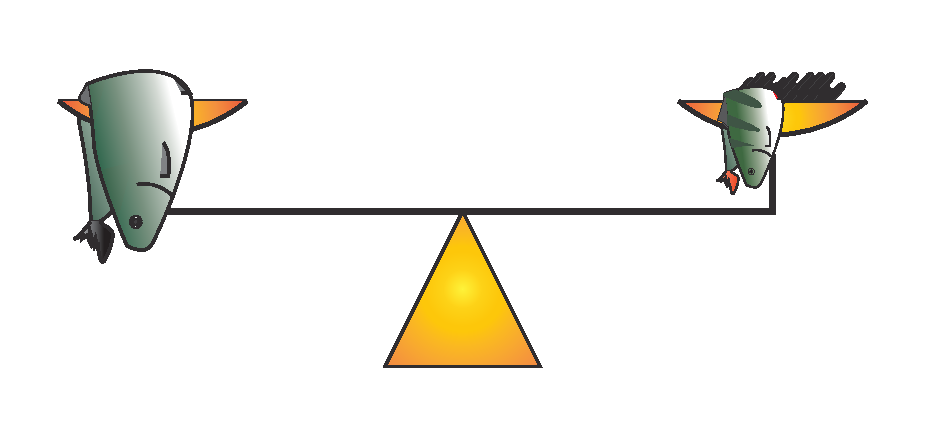
\includegraphics[scale=0.6]{pictures/Kuva10-1-vaaka.pdf} % CC-BY Lilja Tamminen
		%\includegraphics{unused/kala-vaaka.png} % CC-BY Hannu Köngäs
		% FIXME: Hannun piirros on viimeistellympi (smoothit värjäykset jne.), Liljan piirros taas konsistentimpi
		% kirjan muun kuvituksen kanssa. Kumpi jätetään? Nyt päällä Liljan kuva.
	\end{center}
	\begin{esimratk}
		Merkitään lakritsin määrää tuntemattomalla $x$. Tilannetta kuvaa yhtälö $2 = 0,5 + x$.
		Ratkaistaan yhtälö.
		\begin{align*}
			2 &= 0,5 + x &&\text{| $-0,5$} \\
			2 - 0,5 &= x && \\
			1,5 &= x && \\
			x &= 1{,5} &&
		\end{align*}
	\end{esimratk}
	\begin{esimvast}
		Lakritsia on $1,5$ kg.
	\end{esimvast}
\end{esimerkki}

\begin{esimerkki}
	Juna Helsingistä Jyväskylään kulkee $342$ kilometrin matkan kolmessa tunnissa ja $23$ minuutissa tasaista vauhtia.
	$10$ minuuttia junan lähdön jälkeen auto lähtee Helsingistä Jyväskylään kulkien tasaista $100$ kilometrin tuntivauhtia.
	Jyväskylään on Helsingistä maanteitse $272$ kilometriä.
	Kuinka kauan auton lähdöstä on kulunut, kun juna ja auto ovat kulkeneet yhtä suuren osan omista matkoistaan?
	\begin{esimratk}
		Lasketaan aluksi junan nopeus.
		\[ 3 \; \text{h} \; 23 \; \text{min} \; = 12~180 \; \text{s} \]
		\[ \dfrac{342~000 \; \text{m}}{12~180 \; \text{s}} \approx  28,0788 \frac{\text{m}}{\text{s}} \]
		
		Muunnetaan lisäksi auton nopeus yksikköön $\frac{\text{m}}{\text{s}}$ (muuntokerroin $3,6$).
		\[ 100 \frac{\text{km}}{\text{h}} \approx 27,7778 \frac{\text{m}}{\text{s}} \]
		
		$10$ minuuttia on $600$ sekuntia.
		
		Voidaan nyt muotoilla yhtälö käyttäen yksiköitä metri ja sekunti. Tuntemattomana on $t$, aika sekunteina auton lähdöstä.
		\[ \dfrac{28,0788(t+600)}{342000} = \dfrac{27,7778t}{272000} \]
		
		Ratkaistaan yhtälö.
		%Välivaiheselityksiä lisäsi Jaakko Viertiö 2013-11-10
		\begin{align*}
			\dfrac{27,7778t}{272000} &= \dfrac{28,0788(t+600)}{342000} &&\text{| $\cdot{272000}$} &&\text{| $\cdot{342000}$}  \\
			342000 \cdot 27,7778t &= 272000 \cdot 28,0788(t+600) \\
			9500007,6t &= 7637433,6(t+600) \\
			9500007,6t &= 7637433,6t + 4582460160 &&\text{| $-7637433,6t$} \\ 
			1862574t &= 4582460160 &&\text{| $:{1862574}$} \\
			t &\approx 2460,28 \approx 2460
		\end{align*}
		
		Muutetaan yksiköksi minuutit.
		\[ 2460 \; \text{s} \; = 41 \; \text{min} \]
	\end{esimratk}
	\begin{esimvast}
		$41$ minuuttia.
	\end{esimvast}
\end{esimerkki}

\laatikko[Yhtälöiden luokittelu]{
	\begin{description}
		\item[Aina tosi yhtälö] Esimerkiksi yhtälöt $8=8$ ja $x=x$.
		\item[Joskus tosi yhtälö] Esimerkiksi yhtälö $x+4=7$ on tosi, kun $x=3$, ja epätosi muulloin.
		\item[Ei koskaan tosi yhtälö] Esimerkiksi yhtälö $0=1$.
	\end{description}
}

Tärkeimpiä näistä ovat joskus todet yhtälöt. Seuraavaksi on esimerkki, joka osoittaa, kuinka näihin vaihtoehtoisiin tilanteisiin saatetaan päätyä yhtälöä
ratkaistaessa.

\begin{esimerkki}
%Lisännyt Jaakko Viertiö 2013-11-10
	\begin{itemize}
		\item{Yhtälö $3x-12=6(\frac{1}{2}x-2)$ on yhtäpitävä yhtälön $0=0$ kanssa, sillä se saadaan tähän muotoon 
		tekemällä yhtäpitävyyden molemmille puolille aina samat laskutoimitukset. Yhtälön yksinkertaisemmasta esityksestä $0=0$ nähdään, että muuttujan $x$ 
		arvo ei vaikuta yhtälön ratkaisuihin. Toisin sanoen yhtälö on täysin sama, olipa muuttuja $x$ mikä tahansa luku. Yhtälö on siis aina tosi.}
		\item{Yhtälö $3x-11=6(\frac{1}{2}x-2)$ on yhtäpitävä yhtälön $0=1$ kanssa. Jälkimmäisestä muodosta nähdään, ettei yhtälö voi olla tosi millään
		muuttujan $x$ arvolla, sillä yhtälön muodossa $0=1$ ei esiinny muuttujaa $x$. Täten $x$ ei vaikuta yhtälön ratkaisuihin. 
		Yhtälö on siis aina epätosi.}
		\item{Yhtälö $3x-11=6(x-2)$ on yhtäpitävä yhtälön $x=\frac{1}{3}$ kanssa. Yhtälö on siis joskus tosi: täsmälleen silloin kun $x=\frac{1}{3}$.
		Tämä voidaan tarkistaa sijoittamalla yhtälöön $x$:n paikalle arvo $\frac{1}{3}$, jolloin yhtälön vasen ja oikea puoli ovat yhtä suuret.}
	\end{itemize}

\end{esimerkki}


\laatikko[Yleisiä yhtälönratkaisuperiaatteita]{
	\begin{description}
		\item[1)] Kerro tuntematonta sisältävät lausekkeet pois nimittäjistä.
		\item[2)] Yhdistä useat murtolausekkeet yhdeksi laventamalla.
		\item[3)] Yhdistä tuntemattomat.
		\item[4)] Kumoa juuret korottamalla yhtälö puolittain sopivaan potenssiin.
		\item[5)] Sulkuja ei välttämättä aina kannata kertoa auki.
		\item[6)] Yhtälö on ratkaistu vasta, kun jäljellä on enää vain yksi kappale tuntematonta suuretta, ja se sijaitsee yksin omalla puolellaan yhtälöä.
	\end{description}
}

Siirrymme nyt tarkastelemaan tärkeää yhtälöiden lajia, ensimmäisen asteen yhtälöitä.
